\documentclass[10pt]{article}
\usepackage{icmlko}

\icmlmeta{IP 파운데이션 월드모델}{287}{어느 행을 세었나}{한 시간 전 노트가 ``넓힌 판이 벽을 넘긴다''고 썼다 --- 넓힌 판이 더한 행에는 그 축이 없었다}

\begin{document}

\twocolumn[
\icmlheader

\begin{abstract}
노트 286이 오늘 만난 벽 셋이 전부 \textbf{팝업 학습 16행} 하나에서 나온다고
정리하고, 마지막에 좋은 소식을 붙였다 --- 노트 133의 넓힌 판이 그 수를
\textbf{16 $\to$ 73} 으로 늘려 청력 문턱(22)과 채택 검사 ①(30)을 둘 다
넘긴다고. \textbf{틀렸다.} 넓힌 판에서 \texttt{pop\_*} 축이 \emph{관측된}
학습행은 \textbf{17} 이다 --- 넓힌 판이 더한 57행에는 그 파생 필드가 없어서
마스크가 88$\sim$91\% 에서 \textbf{43\%} 로 떨어진다. 그래서 벽을 치웠다고
생각한 판에서 노트 276을 다시 했더니 팝업 \textbf{$+$0.0076}
($t{=}0.54$, 진짜 0개)이다. 좁은 판의 $+$0.0000 에서 거의 안 움직였고,
\textbf{노트 281의 곡선이 이 두 점을 그대로 예측한다}(14행 · 17행 둘 다
문턱 22 아래). 더 나쁜 것은 \textbf{아침에 만든 계기가 이걸 못 잡았다}는
것이다 --- \texttt{hearing.train\_rows} 가 ``라벨 있는 학습행''을 세는데
청력에 필요한 것은 ``\emph{그 축이 관측된} 학습행''이다. 노트 271이 세
행 집합을 갈라 놓고 ``재는 코드를 새로 쓸 때 어느 행을 보는지 이름으로
적으라''고 한 그 자리이고, \textbf{같은 병의 여섯 번째}다. 고쳤다 ---
\texttt{report(..., axis=)} 가 그 축의 마스크까지 보고, 축 없이 부르면
``관측 100\% 가정''이라고 한 줄에 적는다.
\end{abstract}
]

\section{한 시간 전 노트가 틀렸다}

노트 286의 마지막 절이 이랬다.

\begin{quote}\small
노트 133이 이미 만들어 둔 넓힌 판이 팝업 학습을 \textbf{73행}으로 늘린다.
검사 ①(30)과 청력 문턱(22)을 둘 다 넘긴다.
\end{quote}

넓힌 판에서 \texttt{pop\_*} 를 실제로 만들어 보니 이렇다.

\begin{center}\small
\begin{tabular}{lrrr}
\hline
& 좁은 판 & 넓힌 판 & \\
\hline
팝업 전체 행 & 75 & 189 & \\
라벨 있는 학습행 & 16 & \textbf{73} & \\
\texttt{pop\_*} 마스크 & 88$\sim$91\% & \textbf{43\%} & \\
\textbf{그 축 관측 학습행} & \textbf{14} & \textbf{17} & $<$ 22 \\
\hline
\end{tabular}
\end{center}

\textbf{넓힌 판이 더한 57행에는 그 파생 필드가 없다.} 계수 필터를 푼 것이지
문서를 더 읽은 게 아니니 당연하다. \textbf{행은 4.6배가 됐는데 그 축의
행은 셋 늘었다.}

\section{그래서 벽이 안 치워졌다}

\begin{figure*}[t]
\centering
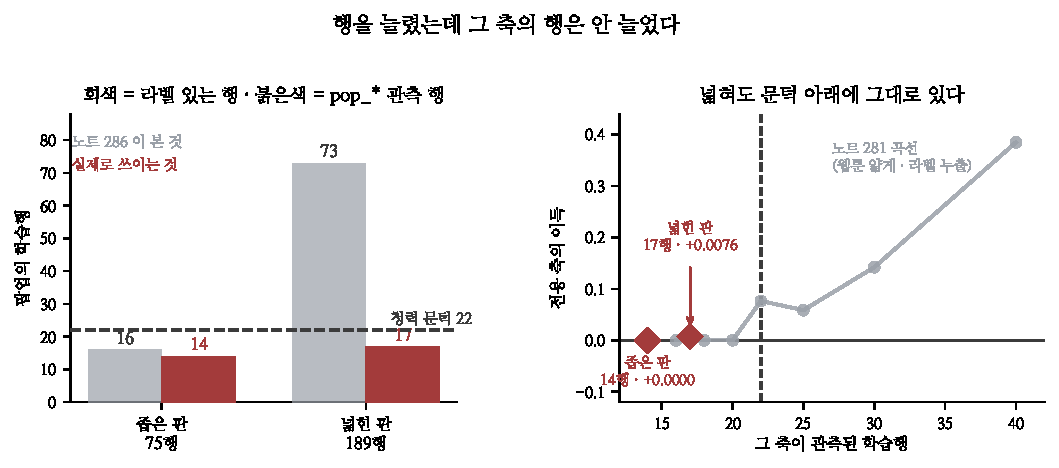
\includegraphics[width=\textwidth]{figs/rows.pdf}
\caption{왼쪽 --- 두 판에서 ``라벨 있는 학습행''과 ``\texttt{pop\_*} 가 관측된
학습행''. 오른쪽 --- 노트 281이 웹툰을 얇게 만들어 그린 곡선 위에 이번 두
점을 얹은 것.}
\end{figure*}

벽을 치웠다고 생각한 판에서 노트 276을 다시 했다.

\begin{center}\small
\begin{tabular}{lrrr}
\hline
& 팝업 전 & 팝업 후 & 차 \\
\hline
좁은 판(노트 276) & 0.3649 & 0.3649 & \textbf{$+$0.0000} \\
넓힌 판 & 0.3582 & 0.3658 & \textbf{$+$0.0076} \\
\hline
\multicolumn{4}{l}{넓힌 판 spread --- 순 $+$0.0003 · \textbf{진짜 0개}} \\
\multicolumn{4}{l}{팝업 짝SE 0.0143 · $t{=}0.54$} \\
\hline
\end{tabular}
\end{center}

\textbf{거의 안 움직였다.} 그리고 이 두 점이 \textbf{노트 281의 곡선 위에
그대로 앉는다} --- 그 노트가 웹툰을 얇게 만들어 훑으며 ``20까지 정확히 0,
22에서 $+$0.0765''를 얻었는데, 여기 14행과 17행이 둘 다 그 왼쪽이다.
\textbf{다른 도메인 · 다른 축 · 다른 판인데 같은 곡선을 따른다.}

\paragraph{$+$0.0076 이 0 이 아닌 것} 노트 281의 곡선은 20까지 정확히 0
이었는데 여기 17행에서 $+$0.0076 이다. $t{=}0.54$ 라 잡음과 못 가른다.
그리고 그 곡선은 \textbf{라벨을 통째로 준 열}로 그린 상한이고 여기는 진짜
축이니, 상한 위에 있을 이유가 없다. \textbf{두 수 다 ``문턱 아래''로 읽는
것이 맞다.}

\section{계기가 못 잡았다}

이게 이 노트에서 제일 아픈 부분이다. \textbf{오늘 아침에 만든
\texttt{lab/hearing.py} 가 이걸 못 잡았다.}

\begin{center}\small
\begin{tabular}{lrl}
\hline
\texttt{hearing.report} & 팝업 학습행 & 판정 \\
\hline
축 무관(옛 판) & 73 & ``듣는다'' \textbf{(틀림)} \\
\texttt{axis="pop\_comp"} & \textbf{17} & ``못 듣는다'' (맞음) \\
\hline
\end{tabular}
\end{center}

\texttt{train\_rows} 가 ``연도 $<$ T 이고 라벨이 있는 행''을 셌다. 그건
\textbf{관측 100\% 인 축에만} 맞는 수다. 청력이 묻는 것은 ``이 열로 가르는
분기가 잎을 채우나''이므로 \textbf{그 열이 관측된 행}을 세야 한다.

\paragraph{같은 병의 여섯 번째} 노트 271이 정확히 이걸 이름 붙여 놨다 ---
행 집합이 셋이다(유보 행 · 라벨 있는 행 · \textbf{그 축 관측 행}). 그때
셋을 세고, 노트 273이 넷째를, 노트 281이 다섯째(\texttt{guards.\_split})를
찾았다. \textbf{여섯째가 오늘 아침 내가 새로 쓴 코드다.}

노트 271이 남긴 규약이 ``재는 코드를 새로 쓸 때 어느 행을 보는지 이름으로
적고, 새 코드의 첫 수치는 행 수를 세어 본다''였다. \textbf{첫 수치의 행
수를 안 셌다} --- 팝업 16행이 문턱 22 아래라 답이 맞아서 그냥 넘어갔다.

\paragraph{고쳤다} \texttt{train\_rows(data, T, axis=)} · \texttt{report(...,
axis=)} 가 그 축의 관측 마스크까지 본다. 축 없이 부르면 한 줄에 \textbf{``축
무관(관측 100\% 가정)''}이라고 적는다 --- 모르는 채로 답을 내지 않게.

\section{그러면 팝업은 어떻게 하나}

노트 286의 결론은 여전히 산다 --- \textbf{세 벽이 팝업 학습 16행 하나에서
나온다.} 바뀐 것은 \emph{손잡이가 이미 있다}는 마지막 문장이다.

\begin{center}\small
\begin{tabular}{lrrl}
\hline
층 & 라벨 학습행 & \texttt{pop\_*} 관측 & 문턱 22 \\
\hline
좁은 판 & 16 & 14 & X \\
넓힌 판 & 73 & \textbf{17} & \textbf{X} \\
\hline
\end{tabular}
\end{center}

\textbf{계수 필터를 푸는 것으로는 안 된다.} 그 축을 늘리려면 \emph{문서를
더 읽어야} 한다 --- 넓힌 판에 들어온 114행의 \texttt{conditions.derived}
를 채우는 일이고, 그건 인제스트 작업이지 축 세트 선택이 아니다.

\paragraph{남은 것}
\begin{center}\small
\begin{tabular}{ll}
\hline
갈래 & 왜 \\
\hline
넓힌 팝업 파생 채우기 & 114행에 \texttt{derived} 를 넣으면 관측 17 $\to$ 70$+$ \\
청력 기록에 축 달기 & 루프가 축별로 적게 \\
관측 100\% 아닌 축 감사 & 다른 축들도 이 오차가 있나 \\
시장팝업 축 관측 & 거기도 마스크 79$\sim$100\% 라 확인 \\
\hline
\end{tabular}
\end{center}

\paragraph{규약} \textbf{``행을 늘렸다''고 쓰기 전에 \emph{어느} 행인지 센다.}
넓힌 판은 라벨 있는 행을 4.6배로 늘렸고 그 축의 행은 셋 늘렸다. 그리고
\textbf{내가 오늘 만든 계기도 오늘 안에 틀린다} --- 아침에 세운 청력 모듈이
저녁에 잘못된 답을 냈고, 잡은 것은 모듈이 아니라 \textbf{실제로 만들어 보고
행을 세어 본 것}이다.

\end{document}
